\documentclass[a4paper]{report}
\usepackage{amsmath,amssymb,amsfonts}\usepackage[left=1in,right=1in,top=1in,bottom=1.5in]{geometry}
\usepackage{graphicx}
\usepackage{layouts}
\usepackage{sectsty}
\usepackage{setspace}
\usepackage[parfill]{parskip}
\usepackage{enumitem}
\usepackage{titlesec}
\titleformat{\chapter}[display]
  {\normalfont\LARGE\bfseries}{}{0pt}{\LARGE}
\titlespacing*{\chapter}{0pt}{-0.5in}{15pt}
\usepackage{gensymb}
\usepackage{mathtools}
\usepackage{url}
\usepackage{verbatim}
\usepackage{siunitx}
\usepackage{physics}
\usepackage{diagbox}
\usepackage[labelfont=bf,font=small]{caption}
\usepackage{subcaption}
\usepackage[]{hyperref}
\usepackage[style=phys,biblabel=brackets]{biblatex}
\usepackage[toc, page]{appendix}
\addbibresource{References.bib}

\begin{document}
\begin{onehalfspace}
\pagenumbering{roman}
\vspace*{0.5in}
\begin{center}
\begin{LARGE}
\textbf{E213 : Analysis of Decays of heavy vector boson $\rm Z^{0}$}\\ 
\end{LARGE}
\bigskip
\bigskip
\textit{A lab report written by}\\
Group P20: Mrunmoy Jena and Ajay Shanmuga Sakthivasan\\
\medskip
\textbf{Supervisor: Martin Angelsmark}\\
\vspace*{5in}
\begin{flushright}
Universit\"{a}t	Bonn\\
\today
\end{flushright}
\end{center}
\tableofcontents
\chapter*{Introduction}
\pagenumbering{arabic}
\addcontentsline{toc}{chapter}{\textbf{Introduction}}

\chapter{Theoretical Background}
%\addcontentsline{toc}{chapter}{\textbf{Theoretical Background}}
\section{The Standard Model- A Brief Overview}
The Standard Model of particle physics which has been one of the most successful and well-tested theories so far, provides the most fundamental description of nature by incorporating the elementary particles and their interactions. These elementary particles are categorized into two families: fermions (having half integer spins) which form matter as we know it, and bosons (with integer spins) serving as mediators of the three fundamental forces. While electromagnetic interactions are mediated by the photon ($\gamma$); strong and weak interactions are mediated by gluons (g) and by $W^{\pm}, Z^{0}$ bosons respectively. A fundamental particle that mediates gravitation has been only postulated theoretically, and is left out of the Standard Model, since the effects of gravity are too weak to play any important role in the realm of particle physics. 

\begin{figure}[h!]
\centering
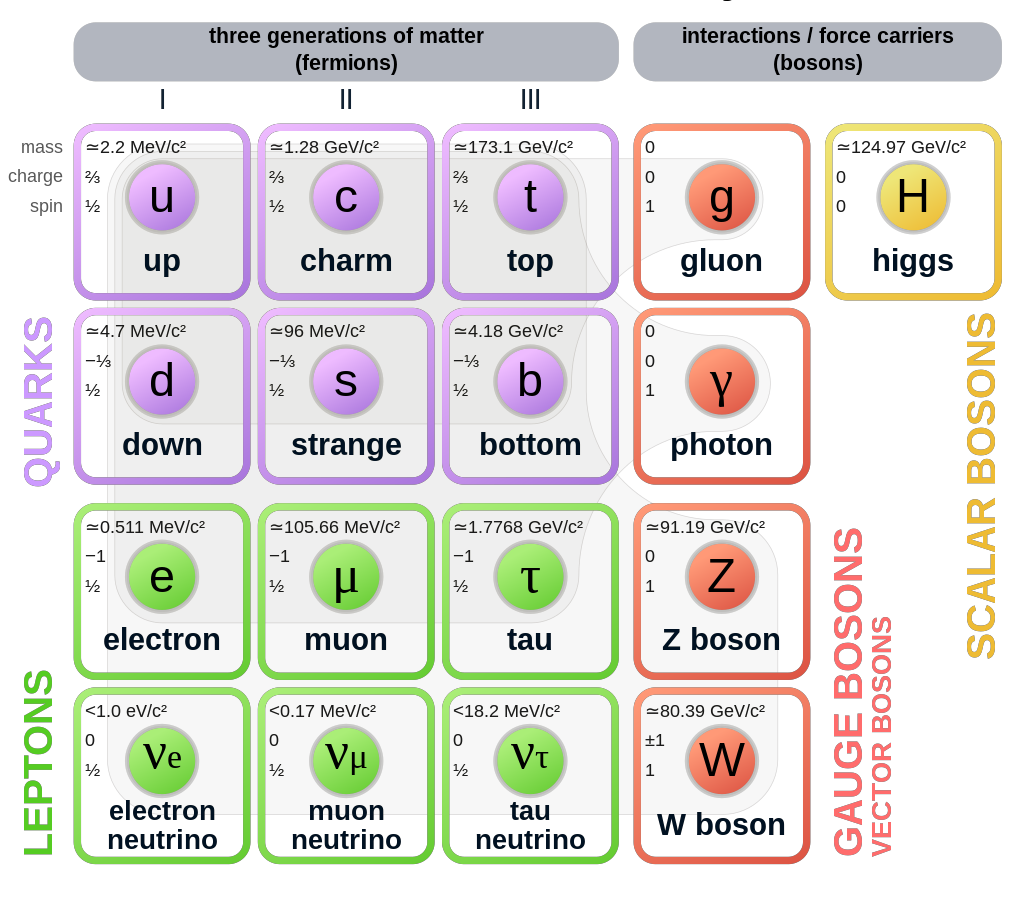
\includegraphics[scale=0.4]{./images/Standard_Model_of_Elementary_Particles.png}
\caption[The Standard Model of elementary particles]{A chart showing the families of elementary particles in the Standard Model \cite{stdmodel}}
\label{fig:StdModel}
\end{figure}

The fermions consists of three generations of quarks and leptons. The quarks have six flavours: up (u), down (d), charm (c), strange (s), top (t) and bottom (b). Similarly, the leptons consist of the electron ($e$), muon ($\mu$) and tau ($\tau$), each having its own associated charge-less and almost massless neutrino ($\nu_{e}$, $\nu_{\mu}$ and $\nu_{\tau}$). Furthermore, each particle in the standard model has its own antiparticle. The quarks are able to form composite particles in either three quark combinations, called baryons ($qqq$/$\bar{q}\bar{q}\bar{q}$) or a quark-antiquark pair, called a meson ($q\bar{q}$). Mathematically, the elementary particles are described as elements of representations of certain symmetry groups. The gauge fields that couple to these particles (i.e. mediate the interactions) arise naturally as a consequence of invariance of their corresponding Lagrangian under local phase transformations \cite{thomson_2013}. As such, the gauge symmetry that governs the Standard Model is given by: $$SU(3)_{\mathrm{Colour}}\times SU(2)_{\mathrm{Left\ chiral}}\times U(1)_{\mathrm{Y}(\mathrm{Weak \ hypercharge})}$$

\section{The Unified Theory of Electromagnetic and Weak Interactions}
Since the experiment deals with verifying some of the properties of the $Z^{0}$ bosons, it is of interest to touch upon the theory of electroweak unification.

While electromagnetism and the theory of weak interactions were formulated separately, it was later on postulated that at higher energies ($\sim$ 246 GeV \cite{pdg-ew}), both these interactions would be unified into a single force. As such, the GSW(Glashow-Salam-Weinberg) electroweak model was developed in the 1960s to describe this unified force. 

One finds that imposing the principle of local gauge invariance on the $SU(2)_{L}$ symmetry group leads to the introduction of three gauge fields: $W^{(1)},\ W^{(2)}$ and $W^{(3)}$ (or $W^{0}$ in some references) \cite{thomson_2013}. The physical $W^{+}$ and $W^{-}$ bosons (that mediate the weak charged current interaction) can be seen as the linear combinations: 
\begin{equation}
W^{\pm}=\dfrac{1}{\sqrt{2}}\left(W^{(1)}\mp W^{(2)}\right)
\end{equation}
However, the $W^{(3)}$ field has no physical interpretation of its own. Therefore an additional symmetry, the $U(1)_{Y}$ group is introduced. The field $B$ (or equivalently $Y^{0}$) arising as a consequence of this new symmetry, similarly does not have a physical meaning on its own. Rather, it was seen that linear combinations of the $W^{(3)}$ ($W^{0}$) and $B$ ($Y^{0}$) fields gives rise to the  photon and the $Z^{0}$ boson:

\begin{equation}
\begin{pmatrix} 
\gamma \\ 
Z^{0} 
\end{pmatrix}
= 
\begin{pmatrix}
\cos \theta_{W} & \sin \theta_{W} \\
-\sin \theta_{W} & \cos \theta_{W} 
\end{pmatrix}
\begin{pmatrix}
B \\
W^{(3)}
\end{pmatrix}
\end{equation}
where $\theta_{W}$ is the weak mixing/Weinberg angle

In addition to this, it is to be noted that the gauge fields $W^{(1),(2),(3)}$ and $B$ have to be massless, in order to respect gauge invariance under local $SU(2)_{L}\times U(1)_{Y}$ gauge transformation. However, the physical gauge bosons $W^{\pm}$ and $Z^{0}$ are predicted to be massive, whereas the photon should remain massless. To explain this, the concept of electroweak spontaneous symmetry breaking was introduced. A massive scalar field (the Higgs field) is introduced, to which these bosons ($W^{\pm}$, $Z^{0}$) must couple to, in order to get their physical masses, while the photon does not interact with it \cite{Dooling:207610}. The intricacies of the Higgs mechanism are not of immediate interest here, and can be understood from standard references \cite{thomson_2013, Griffiths:111880}.

\section{Physics Related to the $Z^{0}$ Resonance}
\subsection{$e^{+}e^{-}$ Interactions}
Before discussing the processes of interest involving $Z^{0}$ production, we first list out the important ways in which $e^{+}e^{-}$ pairs can interact \cite{UB}:
\begin{itemize}
\item $\bm{e^{+}e^{-}\rightarrow e^{+}e^{-}}$: Bhaba scattering (elastic scattering) of $e^{+}e^{-}$ pairs 
\item $\bm{e^{+}e^{-}\rightarrow e^{+}e^{-}f \bar{f}}$: two photon process; $e^{+}e^{-}$ can scatter off of virtual photons, arising out of the incoming $e^{-}$ and $e^{+}$ themselves and these photons can then produce hadrons
\item $\bm{e^{+}e^{-}\rightarrow f \bar{f}}$: Electron-positron pairs annihilate to produce a gauge boson ($\gamma$ or $Z^{0}$), which would in turn produce a fermion-antifermion ($f\bar{f}$) pair. Here $f\bar{f}$ are fermions other than $e^{+}e^{-}$ since that process is already included under Bhaba scattering.
\item $\bm{e^{+}e^{-}\rightarrow \gamma \gamma / \gamma \gamma \gamma}$: An electron-positron pair could also produce two or three photons 

These $e^{+}e^{-}$ interactions are displayed in Figure \ref{fig:eeint}.

\end{itemize}

\begin{figure}[H]
\centering
\begin{subfigure}{0.4\textwidth}
    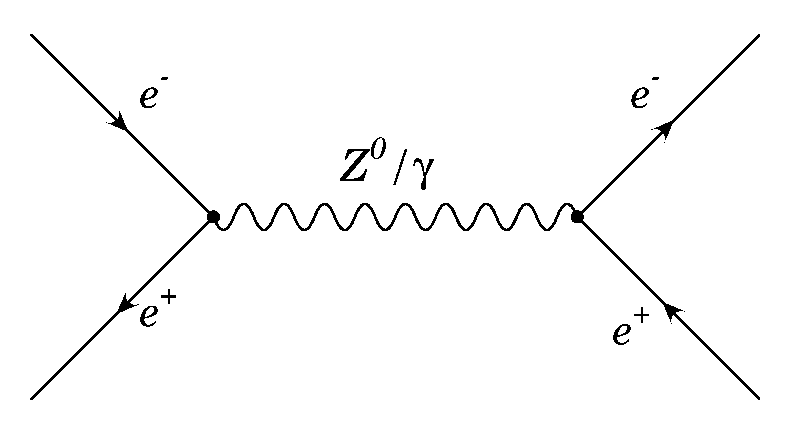
\includegraphics[width=\textwidth]{bhabha-s}
    \caption{$s$-channel Bhaba scattering}
\end{subfigure}
%\hfill
\begin{subfigure}{0.4\textwidth}
    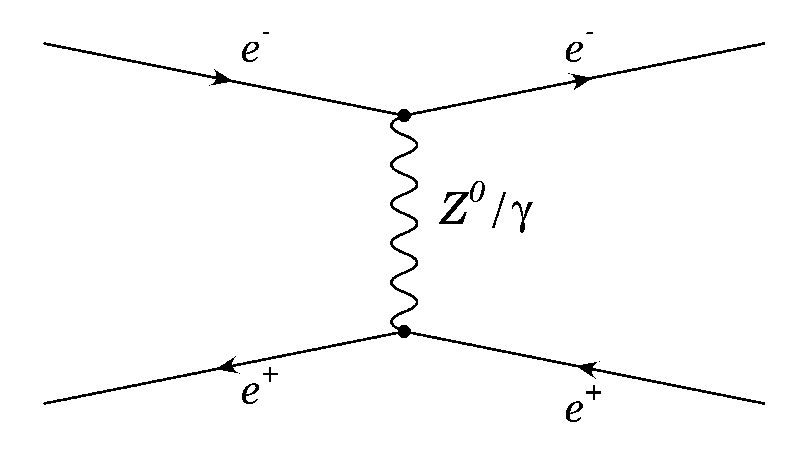
\includegraphics[width=\textwidth]{bhabha-t}
    \caption{$t$-channel Bhaba scattering}
\end{subfigure}
%\hfill
\begin{subfigure}{0.4\textwidth}
\centering
    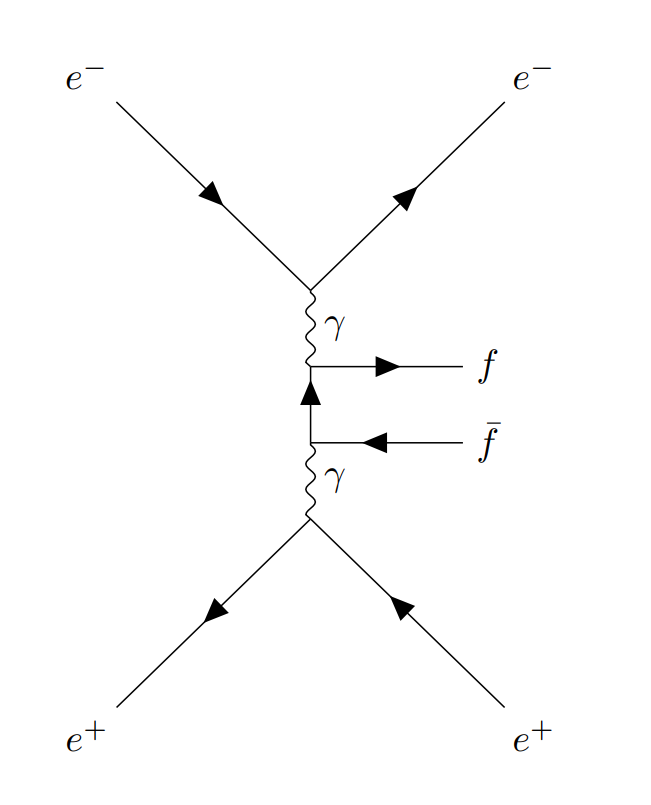
\includegraphics[width=0.9\textwidth]{twophoton}
    \caption{Two photon process}
\end{subfigure}
%\hfill
%\vspace{5em}
\begin{subfigure}{0.4\textwidth}
\centering
    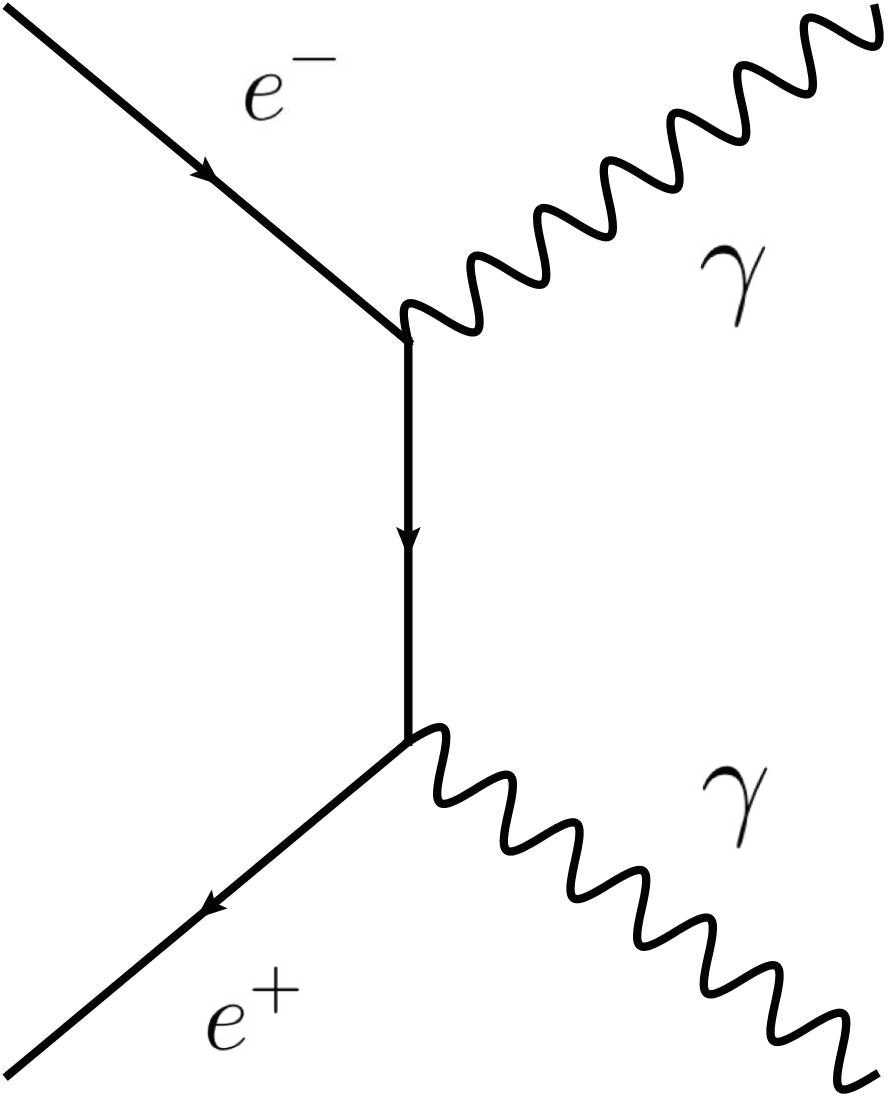
\includegraphics[width=0.7\textwidth]{eeyy}
    \vspace{2em}
    \caption{Production of two photons from $e^{+}e^{-}$ pair}
\end{subfigure}
%\hfill 
\begin{subfigure}{0.45\textwidth}
    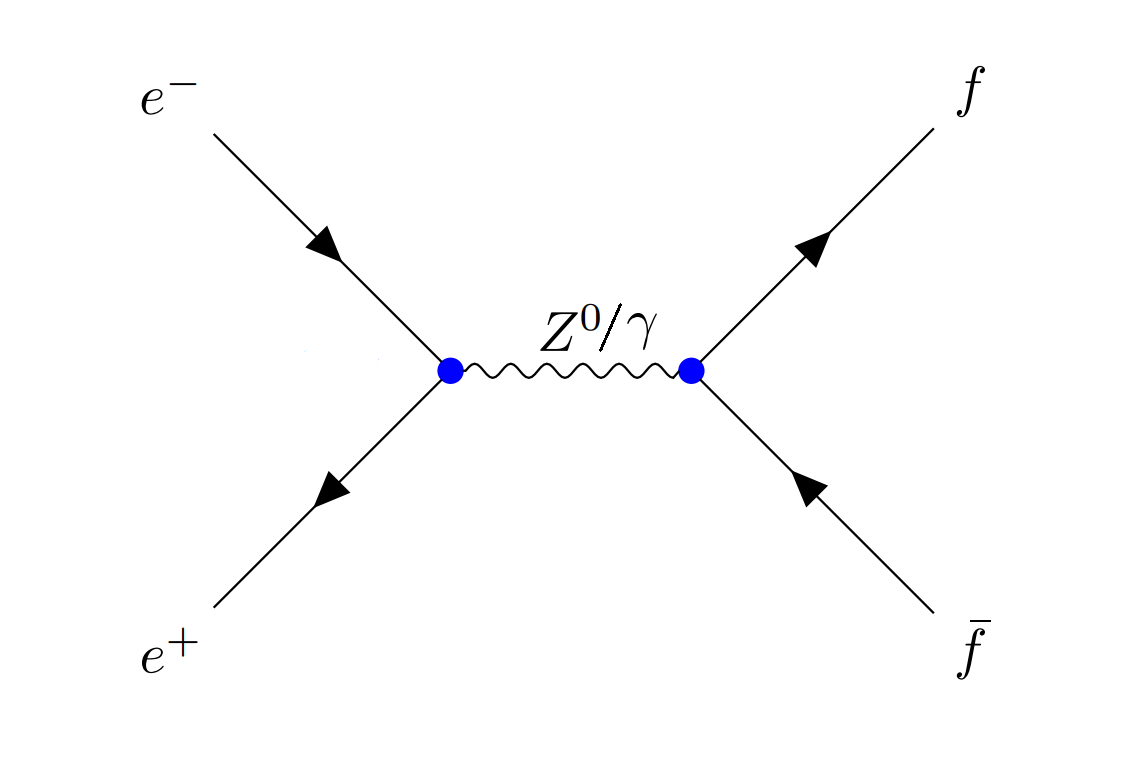
\includegraphics[width=\textwidth]{anihillation}
    \caption{Electron-positron annihilation to $f\bar{f}$}
\end{subfigure}
%\hfill      
\caption[Examples of $e^{+}e^{-}$ interactions]{Examples of $e^{+}e^{-}$ interactions \cite{UB,Janot:2705419,qmdiaries}}
\label{fig:eeint}
\end{figure}

In case of the lowest order $e^{+}e^{-}\rightarrow f \bar{f}$ process, in general, there are contributions to cross section from pure $Z^{0}$, pure $\gamma$ as well as from $\gamma - Z^{0}$ interference terms. However, near center of mass energies close to the $Z^{0}$ resonance, the major contribution to the total cross section is from the pure $Z^{0}$ term.

Additionally, it is easy to see that for the particular case of $e^{+}e^{-}\rightarrow e^{+}e^{-}$ scattering (Bhaba scattering), there is a t-channel contribution in addition to the s-channel component. The cross sections of both these processes have have different angular dependencies \cite{UB}
\begin{align}
\left(\dfrac{d\sigma}{d\Omega}\right)_{s}&\propto (1+\cos^{2}\theta)\\
\left(\dfrac{d\sigma}{d\Omega}\right)_{t}&\propto (1-\cos\theta)^{-2}
\end{align}
This means that while the $s$ channel cross section has a major contribution at large angles (or small values of $\cos\theta$), the $t$-channel contribution increases asymptotically at small angles (or large values of $\cos\theta$). As shall be seen later on, removing the t-channel contribution is an essential step, since we are only concerned with finding the inherent forward-backward asymmetry associated with the $s$-channel processes.

\subsection{Forward-Backward Asymmetry}
\label{FBasymm}
When we consider the $s$-channel processes $e^{+}e^{-}\rightarrow f\bar{f}$, as discussed before, if the process is mediated purely by photons ($\gamma$) then the differential cross section follows the $(1+\cos^{2}\theta)$ dependence and it shows a symmetric dependence on the scattering angle $\theta$. However, for the same process mediated by $Z^{0}$ bosons we find that there is an additional term contributing to the asymmetry:
\begin{equation}
\left(\dfrac{d\sigma}{d\Omega}\right)_{s\ (Z^{0})}\propto a(1+\cos^{2}\theta) + 2b\cos\theta
\end{equation}

From theory of electroweak interactions, this asymmetry (between the number of fermions produced in the forward direction, $\theta>\pi /2$ and the backward direction, $\theta<\pi /2$) can be understood to be arising from the fact that the $Z^{0}$ does not couple equally to right handed and left handed fermions. This becomes more clear by looking at the form of the asymmetry term:
\begin{equation}
b=\left[\left(g_{L}^{e}\right)^{2}-\left(g_{R}^{e}\right)^{2}\right]\left[\left(g_{L}^{f}\right)^{2}-\left(g_{R}^{f}\right)^{2}\right]
\end{equation}
where $g_{L}^{f}$ and $g_{R}^{f}$ signify the coupling of $Z^{0}$ to left handed and right handed fermions respectively. It can be clearly seen that in case the these two couplings had been equal, the asymmetry term would have gone to zero \cite{thomson_2013}.

The forward backward asymmetry factor is given as the ratio:
\begin{equation}
\mathcal{A}_{fb}=\dfrac{\sigma_{F}-\sigma_{B}}{\sigma_{F}-\sigma_{B}}=\dfrac{3b}{4a}
\end{equation}
where $\sigma_{F}$ and $\sigma_{B}$ are the cross sections in forward and backward directions respectively.

It is found that at the resonance of $Z^{0}$ boson, $\mathcal{A}_{fb}$ simplifies to \cite{UB}:
\begin{equation}
\label{eqn:Weinbergangle}
\mathcal{A}_{fb}^{f}\approx 3\left(\dfrac{g_{V}^{f}}{g_{A}^{f}}\right)=1-4\sin^{2}\theta_{W} 
\end{equation}
Thus from the calculation of the forward-backward asymmetry, the ratio of $g_{V}^{f}$ (vector coupling strength between $Z^{0}$ and fermions) to $g_{A}^{f}$ (axial vector coupling strength between $Z^{0}$ and fermions) can be found, which in turn gives us the Weinberg (weak mixing) angle $\theta_{W}$.
\subsection{Background Processes: Radiative Corrections}
In order to test out the predictions of the Standard Model at a very high level of precision, higher order background processes need to be accounted for and as such the corrections made due to these processes are called `radiative corrections'. The following are some of these processes that need to be accounted for \cite{Zedometry}:
\begin{itemize}
\item \textbf{Initial state radiation (ISR):} The radiation of photons in the initial state lead to decrease in the centre of mass energy and thus affects the $Z^{0}$ resonance peak parameters. This leads to a peak height reduction by upto 25 \%, shift of peak to higher energy and increase in full width at half maximum (FWHM). 
\item \textbf{Final state radiation (FSR):} When photons or gluons are radiated in the final state, it is found that partial widths increase by the corresponding factors:
\begin{equation}
\Delta_{QED}=1+\dfrac{3}{4}\dfrac{Q_{f}^{2}\alpha(m_{Z}^{2})}{\pi}\ ;\ \Delta_{QCD}\approx 1+\dfrac{\alpha_{s}(m_{Z}^{2})}{\pi}
\end{equation}
\item \textbf{QED vacuum polarization:} The production of $e^{+}e^{-}$ pairs from vacuum makes the QED coupling constant scale dependent: 
\begin{equation}
\alpha(0)\rightarrow \alpha(s)=\dfrac{\alpha{0}}{1-\Delta \alpha(s)}
\end{equation}
It has been shown that the imaginary part of $\Delta \alpha(s)$ has an influence on the $\gamma / Z^{0}$ interference term.
\item \textbf{Electroweak corrections:} Further contributions also arise from virtual processes such as higher order loops in $Z^{0}$ propagator and vertex corrections.


Some instances of these radiative corrections are shown in Figure \ref{fig:backfig}
\end{itemize}

\begin{figure}[H]
\centering
\begin{subfigure}{0.45\textwidth}
    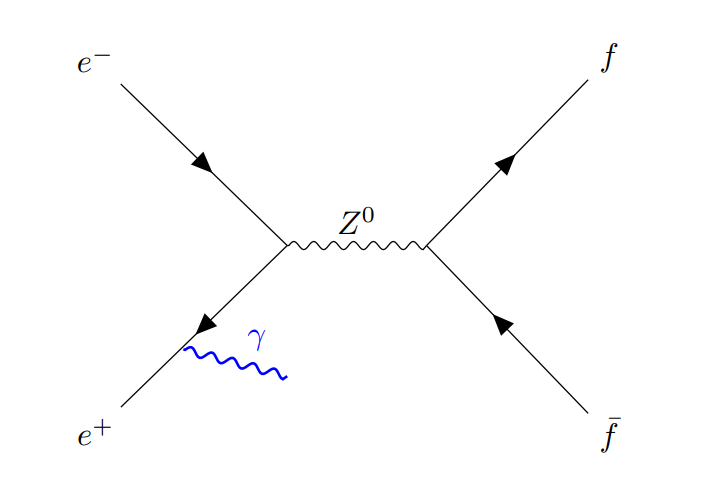
\includegraphics[width=\textwidth]{background1}
    \caption{Initial state radiation (ISR)}
\end{subfigure}
%\hfill
\begin{subfigure}{0.45\textwidth}
    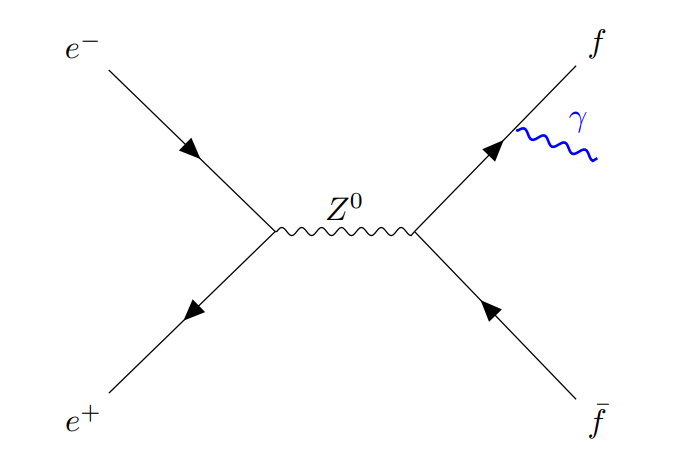
\includegraphics[width=\textwidth]{background2}
    \caption{Final state radiation (FSR)}
\end{subfigure}
%\hfill
\begin{subfigure}{0.45\textwidth}
    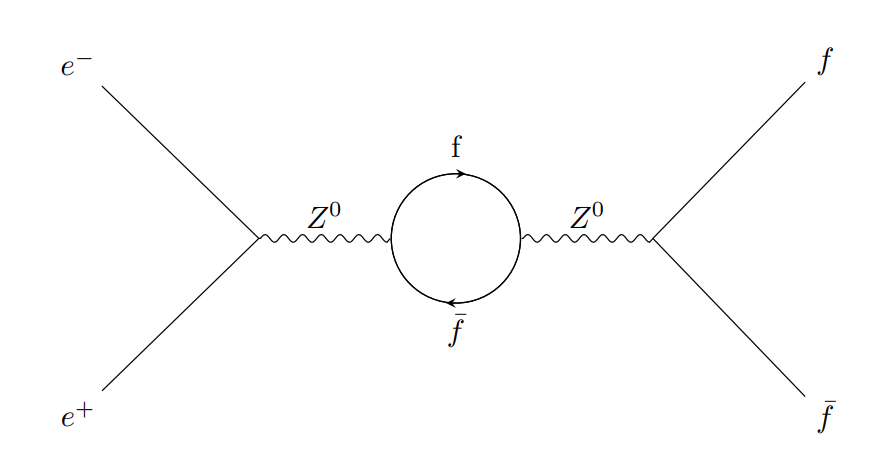
\includegraphics[width=\textwidth]{background3}
    \caption{$Z^{0}$ propagator correction}
\end{subfigure}
%\hfill
\begin{subfigure}{0.45\textwidth}
    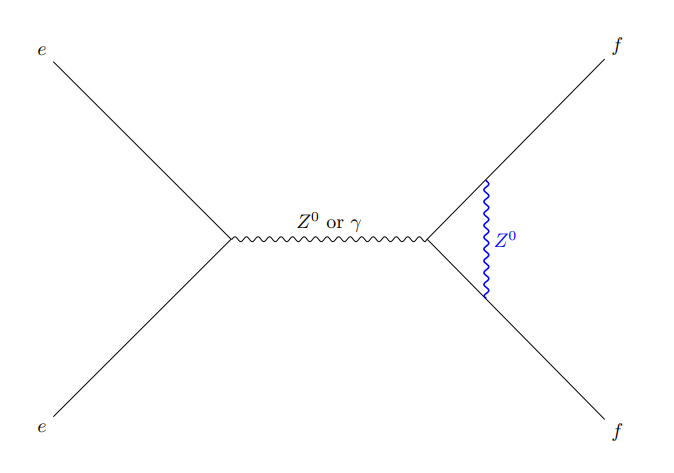
\includegraphics[width=\textwidth]{background4}
    \caption{$Z^{0}$ vertex correction}
\end{subfigure}       
\caption[Examples of radiative corrections]{Examples of radiative corrections \cite{UB}}
\label{fig:backfig}
\end{figure}

\subsection{Mass and Width of the $Z^{0}$ Boson - The Breit Wigner Distribution}
From the theory of electroweak interactions, it is known that the contribution the $Z^{0}$ boson exchange propagator to the matrix element (in s-channel processes) can be given by:
\begin{equation}
\mathcal{M}_{Z^{0}}\propto \dfrac{g_{Z^{0}}^{2}}{q^{2}-m_{Z^{0}}^{2}}=\dfrac{g_{Z^{0}}^{2}}{s-m_{Z^{0}}^{2}}
\end{equation}
We one can see from this dependence that around the $Z^{0}$ resonance ($\sqrt{s}\sim  m_{Z^{0}}$), the propagator diverges \cite{thomson_2013}. In order to correct for this, it is necessary to introduce a modification in the propagator for a decaying state. When an unstable particle has a decay rate $\Gamma$, its wavefunction gets modified to:
\begin{equation}
\psi\propto e^{-imt}\rightarrow e^{-imt}e^{-\Gamma t/2}
\end{equation} 
which is equivalent to introducing an additional imaginary term in the mass:
\begin{equation}
m\rightarrow m-i\dfrac{\Gamma}{2}
\end{equation}
Accordingly, the $Z^{0}$ propagator then changes to:
\begin{equation}
\dfrac{1}{s-m_{Z^{0}}^{2}}\rightarrow \dfrac{1}{s-{\left(m_{Z^{0}}-i\Gamma_{Z^{0}}/2\right)}^{2}} 
\end{equation}
On simplifying this result, taking the spin averaged matrix element and inserting the appropriate pre-factors, the complete form of the cross section in the process $e^{+}e^{-}\rightarrow Z^{0}\rightarrow f\bar{f}$ is given by:
\begin{equation}
    \sigma_f (s) = \frac{12\pi}{M_Z^2} \frac{s \Gamma_e \Gamma_f}{(s-M_Z^2)^2 + \left(\frac{s\Gamma_Z}{M_Z}\right)^2} (\hbar^2 c^2),
\end{equation} 
The probability distribution that characterizes the dependence of this cross section on the centre of mass energy is called the Breit-Wigner distribution. This distribution is shown in Figure \ref{fig:BWdist}.

\begin{figure}[H]
\centering
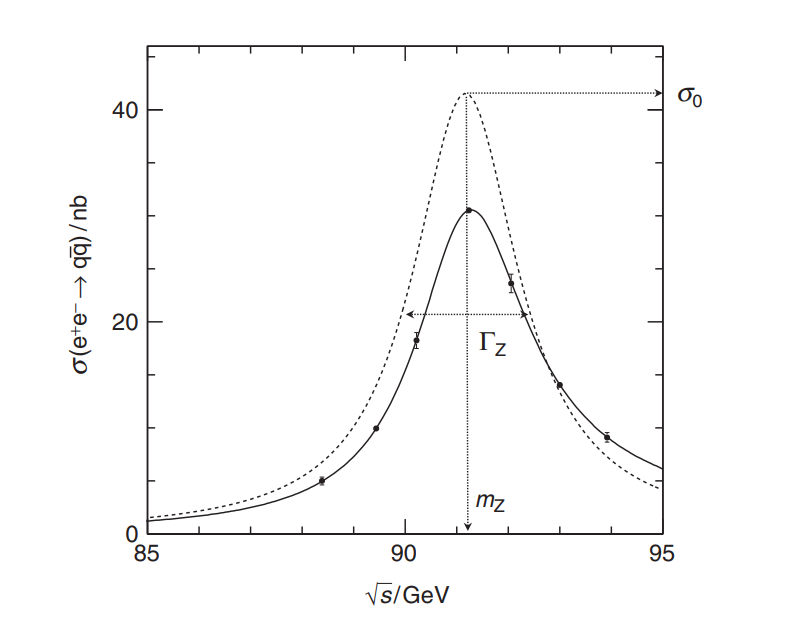
\includegraphics[width=0.6\textwidth]{BWdist}
\caption[Breit Wigner distribution of the cross section for $e^{+}e^{-}\rightarrow q\bar{q}$ process]{The Breit Wigner distribution of the cross section for $e^{+}e^{-}\rightarrow q\bar{q}$ process at centre of mass energies around the $Z^{0}$ resonance (the dashed and solid curves are the distribution after and before corrections for initial state radiation). \cite{thomson_2013}}
\label{fig:BWdist}
\end{figure}
As can be seen from the figure, at the $Z^{0}$ resonance, the physical parameters of the $Z^{0}$ can easily be extracted. For example, the mass of the $Z^{0}$ would simply be the value on the $x$ axis where this peak occurs, its decay width can be found from the full width at half maximum (FWHM) of the curve, and reading off the $y$ value at the resonance peak gives us the resonant cross section. This will in fact be one of the important tasks of the present experiment.

\section{LEP Experiment and the OPAL Detector}
The Large Electron Positron Collider (LEP) was built at CERN, with one of its major goals being making high precision measurements of the parameters of the $Z^{0}$ boson, such as its mass, decay width and angular distributions of final state particles produced from $Z^{0}$ decays. As such, for most of its period of operation from 1989 to 1995, it produced $e^{+}e^{-}$ collisions at centre of mass energies very close to the $Z^{0}$ resonance and about 17 million $e^{+}e^{-}\rightarrow Z^{0}$ events were recorded in this duration \cite{thomson_2013}. The collisions took place at four different points in the circular collider, and hence four such detectors were used in this experiment: ALEPH (Apparatus for LEP PHysics), DELPHI (DEtector with Lepton, Photon and Hadron Identification), L3 (Third LEP experiment) and OPAL (Omni-Purpose Apparatus for LEP). 

The components of the OPAL detector shall be described in further detail in this Section, since this experiment focuses on analysis of data collected by the OPAL.

\subsection{The OPAL Detector and its Components}
\begin{figure}[H]
\centering
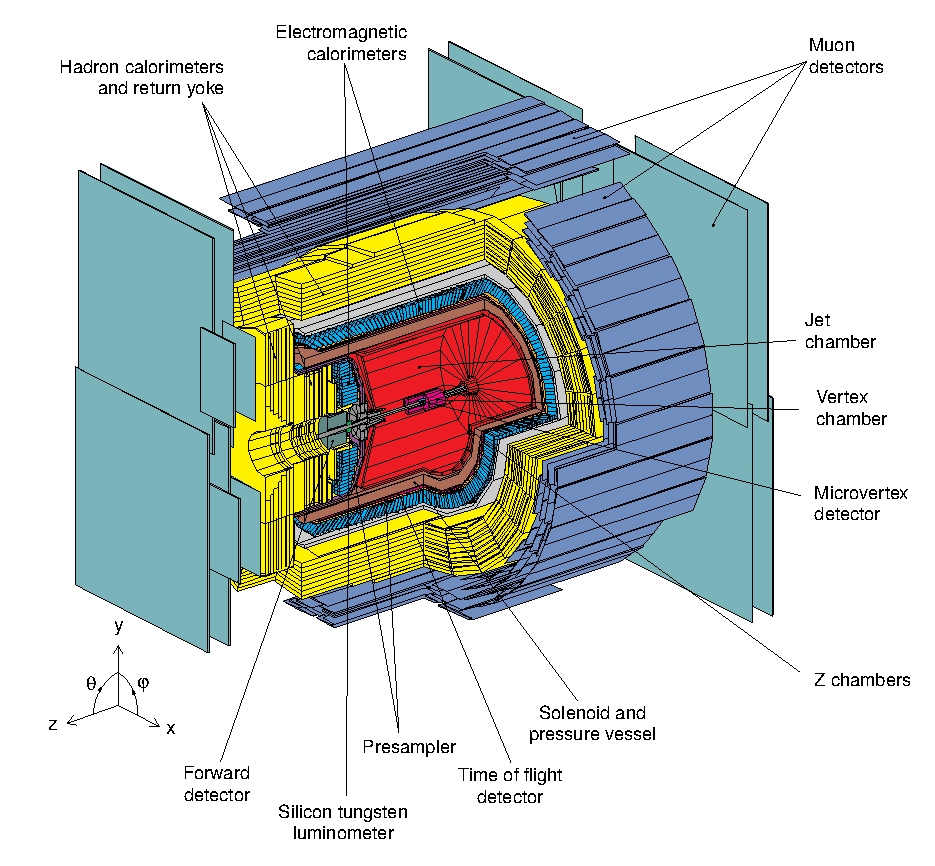
\includegraphics[width=0.69\textwidth]{OPAL1}
\caption[The OPAL Detector and its various components]{The OPAL Detector and its various components \cite{OPAL}}
\label{fig:OPAL}
\end{figure}

For analysis of events arising from this detector, a right handed coordinate system is followed. The origin is fixed at the point where $e^{+}e^{-}$ collisions take place, the $x$ axis points horizontally in the direction of the center of the LEP, while the z axis is defined to lie along along the beam path and the y axis is then just perpendicular to the $x-z$ plane as usual. $\theta$, the polar angle is the angle between the $y$ and $z$ axes and the azimuthal angle $\phi$ is measured counterclockwise between the $x$ and $y$ directions. The OPAL detector and this coordinate system is displayed in Figure \ref{fig:OPAL}.

Starting from the origin, as the $e^{+}e^{-}$ collision products fly outwards, various detector components are encountered which serve to detect the type and various characteristics of the final state particles. These primary detector components are discussed here in brief \cite{UB,1991275}:
\begin{itemize}
\item \textbf{Vertex detector:} This is a type of drift detector that surrounds the central beam pipe and plays a key role in locating vertices of short-lived decay products and also helps in improving the momentum resolution. It has dimensions of 1 m in length and measures 470 mm across (diameter), layered with 36 axial cells that measure positions in the $r-\phi$ plane.  
\item \textbf{Jet chamber:} This is again a cylindrical drift chamber with a good spatial and track resolution, designed in a manner so as to efficiently record events associated with jets. Inside this chamber, there are 24 sectors, each of which contains 159 sensing wires, arranged parallel to the beam axis. Beside the anode wires, there are alternating cathode wires positioned in between the potential and anode wires. The coordinates of the decay particles are obtained from parameters such as the positions of the wires and the drift time. Moreover, the signals from these wires determine the energy loss $dE/dx$ of charged particles in this region.
\item \textbf{$\mathbf{z}$ chambers:} As the name suggests, the $z$ chambers serve the purpose of locating the $z$ coordinates of decay particles when they leave the jet chamber. As such they are helpful in improving the resolutions of the polar angle and invariant mass distributions of charged particles. Consisting of 24 drift chambers, subdivided into 8 cells each, a high $z$ resolution of 100-200 $\mu$m is achieved by these chambers.
\item \textbf{Solenoid:} The solenoid surrounds the detectors discussed so far (collectively called the central detector) and generates a uniform magnetic field of 0.435 T along the beam direction. The magnetic field makes the charged particles follow a helical path in the central detectors and therefore is essential to measure their momenta. 
\item \textbf{Time of flight (TOF) system:} The role of the TOF system is to generate signals (light from a total of 160 scintillation chambers) that trigger the detector and to identify charged particles in the range of 0.6 to 2.5 GeV. Further it is useful in rejecting cosmic rays.
\item \textbf{Electromagnetic calorimeter (ECAL):} This detector is made up of 9440 blocks of lead glass. The geometry of this detector is in the form of a barrel around the jet chamber with two endcaps, covering a total of 98 \% of the solid angle. Particles such as photons, electrons and positrons deposit all of their energy in the ECAL either through Bremsstrahlung ($e^{+}$ or $e^{-}$ emitting a photon) or by pair production (a photon giving rise to an $e^{+}e^{-}$ pair). Hadrons on the other hand, do deposit some of their energy here (in the form of electromagnetic showers), but mostly don't come to a stop in the ECAL. The reason for choosing lead glass for the ECAL is that the material provides an excellent resolution of:
\begin{equation}
\left(\dfrac{\sigma_{E}}{E}\right)_{\rm{ECAL}}\approx \dfrac{5 \%}{\sqrt{E}}
\end{equation}
\item \textbf{Hadron calorimeter (HCAL):} This detector has a similar geometry to that of that of ECAL and serves to detect mesons and baryons. In addition to ionisation energy loss, hadrons also undergo strong interaction with the nuclei that they encounter. As such there can be numerous decay products in the associated hadronic showers. Since the decay products travel significant distances between any two nuclear interactions, the HCAL occupies much more volume of the detector than ECAL and is made up of absorber material with a high density (iron slabs in this case). Because of the uncertainties in determining the amount of energy lost electromagnetically and in the energy loss in nuclear interactions, the energy resolution for the HCAL is poor compared to that of the ECAL:
\begin{equation}
\left(\dfrac{\sigma_{E}}{E}\right)_{\rm{HCAL}}\approx \dfrac{120 \%}{\sqrt{E}}
\end{equation} 
\item \textbf{Muon detector:} Outside the HCAL, lie four layers of muon detectors. The muon detector provides a coverage of almost the entire solid angle of 4$\pi$ and has a barrel region and two endcap regions, similar to the ECAL and HCAL. The detection probability of muons in this detector is very high ($\sim 100 \%$) because almost all of the other decay products have either been absorbed in the ECAL or in the HCAL.
\end{itemize}


\chapter{Pre-Lab Exercises}
%\addcontentsline{toc}{chapter}{\textbf{Pre-Lab Exercises}}
In this chapter, we have provided our solutions to some theoretical questions that were needed to be solved before conducting the experiment. All the equations and standard values of parameters used to calculate the numerical results for these exercises are taken from \cite{UB}, unless mentioned otherwise.
\section{Calculation of partial decay widths for $Z^{0}\rightarrow f\bar{f}$}
In this exercise, we are required to calculate the partial decay widths of $Z^{0}\rightarrow f\bar{f}$; where $f\bar{f}$ represent the following fermion-antifermion pairs : (i) $e^{+}e^{-}$ (ii) $\mu^{+}\mu^{-}$ (iii) $\tau^{+}\tau^{-}$ (iv) $q\bar{q}$, where $q$ represents all the flavours of quarks (except for t quark, because it is too heavy ($M_{t}\approx 172.76$ GeV \cite{Zyla:2020zbs}) to be produced from $Z^{0}$ decays). The partial decay widths have been calculated with the following formula:
\begin{equation}
\Gamma_{f}=\dfrac{N_{c}^{f}\sqrt{2}}{12\pi}G_{F}M_{Z}^{3}\left(\left(g_{V}^{f}\right)^{2}+\left(g_{A}^{f}\right)^{2}\right)
\end{equation}
where:
\begin{description}
\item $N_{c}^{f}$: colour factor, (1 for leptons, 3 for quarks)
\item $G_{F}=1.16637\times 10^{-5}\mathrm{GeV}^{-2}$, Fermi's constant 
\item $M_{Z}=91.182$ GeV, mass of $Z^{0}$ boson
\item $g_{V}^{f}=I_{3}^{f}-2Q_{f}\sin^{2}\theta_{W}$, vector coupling strength of $Z^{0}$ to fermions
\item $g_{A}^{f}=I_{3}^{f}$, axial-vector coupling strength of $Z^{0}$ to fermions
\item $Q_{f}$: electric charge of fermion $f$
\item $I_{3}$: third component of weak isospin
\item $\sin^{2}\theta_{W}=0.2312$, $\theta_{W}$ is the Weinberg (weak-mixing) angle
\end{description}

\begin{table}[h!]
\centering
\begin{tabular}{|c|c|c|c|c|c|c|c|}
\hline
\textbf{Fermion} & $\mathbf{Q_{f}}$ & $\mathbf{I_{3}^{f}}$ & $\mathbf{g_{V}^{f}}$ & $\mathbf{g_{A}^{f}}$ & $\mathbf{N_{c}^{f}}$ & $\mathbf{\Gamma_{f}^{(calc)}}$ \textbf{(MeV)} & $\mathbf{\Gamma_{f}^{(ref)}}$ \textbf{(MeV)}\\
\hline
$e^{-}, \mu^{-}, \tau^{-}$ & -1 & -0.5 & -0.0376 & -0.5 & 1 & 83.89 & 83.8\\
\hline
$u,c$ & 2/3 & 0.5 & 0.1917 & 0.5 & 3 & 285.34 & 299\\
\hline
$d, b, s$ & -1/3 & -0.5 & -0.3459 & -0.5 & 3 & 367.84 & 378\\
\hline
$\nu_{e}, \nu_{\mu}, \nu_{\tau}$ & 0 & 0.5 & 0.5 & 0.5 & 1 & 165.85 & 167.6\\
\hline
\end{tabular}
\caption{Parameters $Q_{f}, I_{3}^{f}, g_{V}^{f}, g_{A}^{f}, N_{c}^{f}$ for various fermion pairs and their partial decay widths}
\label{partialdecays}
\end{table}

The calculated partial decay widths for the required fermion pairs have been listed under $\Gamma_{f}^{(calc)}$ in Table \ref{partialdecays}. Further, the reference \cite{UB} values of partial decay widths for the same fermion pairs are listed under $\Gamma_{f}^{(ref)}$ for comparison. 

One finds that calculated values of partial decay width for the lepton pairs are in close agreement with the literature value, deviating by about 0.1\% to 1\%. The slight deviation could be caused because the $\gamma\rightarrow f\bar{f}$ term \cite{Ver} and interference terms have been neglected. In case of the quarks, the deviations from the reference values are higher ($\sim$ 2.7\% to 4.6\%). This may be due to the fact that additionally, the effect of strong interactions have not been accounted for in our calculations \cite{Anna}.

\chapter{Analysis}
\section{Part I: Analysis of Event Displays}

\section{Part II: Statistical Analysis of $Z^0$ Decays}
In the previous subsection, we carried out an analysis based on event displays. This was possible because we did not have a lot of events to work with. Obviously, such an analysis would prove to be futile if we try to carry it out on a large set of data. Analysis of large sets of data would be the primary discussion of this subsection. We use the software, $ROOT$ to analyse the data on a statistical basis. \textit{ROOT} works with \textit{.root} files, which contain all the information in a tree-like structure, called \textit{ntuple}. The contents of the \textit{ntuple} are,
\begin{itemize}
    \item RUN: Run number
    \item EVENT: Event number
    \item NCHARGED: Number of charged tracks
    \item PCHARGED: Total scalar sum of track momenta
    \item E\_ECAL: Total energy in electromagnetic calorimeter
    \item E\_HCAL: Total energy in hadronic calorimeter
    \item E\_LEP: LEP beam energy ($=\sqrt{s}/2$)
    \item COS\_THRU: cos(polar angle) between beam axis and thrust axis
    \item COS\_THET: cos(polar angle) between incoming positron and outgoing positive particle
\end{itemize}
We also have two categories of data, each containing a lot of \textit{ntuples},
\begin{itemize}
    \item Monte Carlo (MC): These correspond to the ``\textit{pure}'' events from the previous subsection. These are simulated - detector response to a calculated outgoing momentum four-vector for a specific process.
    \item Data: These correspond to the ``\textit{mixed}'' events from the previous subsection. These are real life data recorded with the OPAL detector at specific energies around the $Z^0$ resonance maximum.
\end{itemize}
\textit{ROOT} can be used to set cuts on the above variables in a data and get histograms of different variables. This allows for a statistical analysis of the data. All the above information can be found in \cite{UB}.

\subsection{Refining the cuts}
As mentioned previously, we have two categories of data. There are four Monte Carlo (MC) data, one for each of the decay channels. There are six real world data and we will be using \textit{data6.root} for our analysis in the following parts. Analysis of event displays already gave us an idea of what cuts to use, to extract the different channels. Our first step here will be to test our cuts on the MC data and check how they fare. And the second step will be to refine the cuts a little so that we are better able to extract different channels.\\
When it comes to $e^-e^+$ final state decay channel, we would like to exclude t-channel events. This is because t-channel is possible only in the mode and for the sake of consistency, we would like to limit ourselves to only s-channel. From theory\cite{UB}, we know that the t-channel dominates at large $cos\theta$. By introducing a new cut to exclude events with large $cos\theta$, we eliminate a most of the t-channel events. But this also means that we are eliminating some of the s-channel events. To account for this, we multiply the observed events after applying the modified cuts with correction factor. This correction factor is given by,
\begin{equation}
    \delta = \frac{\int_{-1}^1 (1 + x^2) dx}{\int_{-0.9}^{0.5} (1 + x^2) dx} \approx 1.5829.
\end{equation}
This factor is arrived at from theory, which gives the behaviour of s-channel as proportional to $(1 + cos^2\theta)$ and the integral limits are correspond to the $cos\theta$ values which we exclude.\\
When it comes to $\mu^-\mu^+$ final state decay channel, we observed a lot of events with \textit{PCHARGED} equal to exactly $0$. These events are not physical. Hence we apply a cut to eliminate such events. In the cases of $e^-e^+$ and $\mu^-\mu^+$, we also exclude $cos\theta$ values very close to $1$ and $-1$, as the detector resolution is far from perfect close to the beam axis. To summarise, we have the following additions - $cos\theta \in [-0.9, 0.5]$, to remove t-channel events in the case of $e^-e^+$, $PCHARGED > 0$, to exclude unphysical events in the case of $e^-e^+$ and $cos\theta \in [-0.9, 0.9]$, to eliminate low resolution events in the cases of $e^-e^+$ and $\mu^-\mu^+$. Interestingly, the channels $\tau^-\tau^+$ and $q\bar{q}$ did not require any additional global cuts. But, we did add the cut $cos\theta \in [-1, 1]$ to remove any unphysical events. Analysis done with \textit{ROOT} on the $e^-e^+$ MC can be found in the appendix, \ref{fig:global-ee}, \ref{fig:eecutee}, \ref{fig:mmcutee}, \ref{fig:ttcutee} and \ref{fig:qqcutee}. Analysis on the other MC files and ultimately the data file are done similarly.\\
After testing our cuts, we arrive at the conclusion that we don't need any further refinements other than the additions mentioned above. With these additions, we go about analysing \textit{data6.root}. The raw data of observed events using our cuts is given in the table \ref{table:eventsdata6} below. Note that the correction factor has not been applied to the $e^-e^+$ event numbers but it is used in our latter calculations. The event numbers are exactly what we get after applying all the cuts appropriately.

\begin{table}[!h]
\centering
\resizebox{\columnwidth}{!}{
\begin{tabular}{cccccc}
\hline
\multicolumn{1}{|c|}{}               & \multicolumn{5}{c|}{Number of observed events}                                                                                                                                                                                                                    \\ \hline
\multicolumn{1}{|c|}{MC Sample}      & \multicolumn{1}{c|}{$e^-e^+$ cuts} & \multicolumn{1}{c|}{$\mu^-\mu^+$ cuts} & \multicolumn{1}{c|}{$\tau^-\tau^+$ cuts} & \multicolumn{1}{c|}{$q\bar{q}$ cuts} & \multicolumn{1}{c|}{\begin{tabular}[c]{@{}c@{}}Total \\ (incl. global cuts, if any)\end{tabular}} \\ \hline
\multicolumn{1}{|c|}{$e^-e^+$}       & \multicolumn{1}{c|}{18835}         & \multicolumn{1}{c|}{0}                 & \multicolumn{1}{c|}{378}                 & \multicolumn{1}{c|}{0}               & \multicolumn{1}{c|}{56720}                                                                        \\
\multicolumn{1}{|c|}{$\mu^-\mu^+$}   & \multicolumn{1}{c|}{0}             & \multicolumn{1}{c|}{76209}             & \multicolumn{1}{c|}{8599}                & \multicolumn{1}{c|}{0}               & \multicolumn{1}{c|}{89887}                                                                        \\
\multicolumn{1}{|c|}{$\tau^-\tau^+$} & \multicolumn{1}{c|}{26}            & \multicolumn{1}{c|}{35}                & \multicolumn{1}{c|}{71131}               & \multicolumn{1}{c|}{135}             & \multicolumn{1}{c|}{79214}                                                                        \\
\multicolumn{1}{|c|}{$q\bar{q}$}    & \multicolumn{1}{c|}{0}            & \multicolumn{1}{c|}{0}                & \multicolumn{1}{c|}{173}                  & \multicolumn{1}{c|}{92164}            & \multicolumn{1}{c|}{98563}                                                                                             \\ \hline
\end{tabular}
}
\caption{Number of events with different cuts applied to each of the MC data.}
\label{table:eventsdata6}
\end{table}

\subsection{Efficiency Matrix}
The efficiency matrix is a measure of how efficient the cuts are at extracting the different decay channels. If we consider the actual event numbers of the different channels as a $4 \times 1$ matrix, the efficiency matrix will be a $4 \times 4$ matrix and ideally, it should be a unit matrix. In this case, the event numbers observed matches the actual event numbers. But this is not the case usually. We should aim to achieve an efficiency matrix with diagonal elements as close to $1$ as possible and the off-diagonal elements as close to $0$ as possible. The efficiency matrix elements are given by\cite{UB},
\begin{equation}
    \epsilon_{ij} = \frac{N^{i, cut}_j}{N^{j, all}_j}.
\end{equation}
For example, $\epsilon_{12}$ corresponds to $e^-e^+$ cuts applied to $\mu^-\mu^+$ events divided by the total observed $\mu^-\mu^+$ events. Note that we construct the $4 \times 1$ matrix in the following order - $e^-e^+$ events, $\mu^-\mu^+$ events, $\tau^-\tau+$ events and $q\bar{q}$ events. With this efficiency matrix, one could extract the actual event numbers as follows,
\begin{equation}
    N_{obs} = \epsilon N_{actual} \implies N_{actual} = \epsilon^{-1} N_{obs}.
\end{equation}
This gives us an efficiency matrix,
\begin{equation}
    \epsilon = 
    \begin{pmatrix}
        5.26 \times 10^{-1} & 0 & 3.28 \times 10^{-4} & 0 \\
        0 & 8.48 \times 10^{-1} & 4.42 \times 10^{-4} & 0 \\
        6.66 \times 10^{-3} & 9.57 \times 10^{-2} & 8.98 \times 10^{-1} & 1.76 \times 10^{-3} \\
        0 & 0 & 1.70 \times 10^{-3} & 9.35 \times 10^{-1}
    \end{pmatrix}.
\end{equation}
Given a cut, whether or not a particular event passes it can be modelled with a binomial distribution, just like modelling a coin toss. In the limit when such an ``experiment'' is conducted on large sample size, the probability mass function of the binomial distribution can be approximated by a normal distribution. In which case, the standard deviation is given by,
\begin{equation}
    \Delta \epsilon_{ij} = \sqrt{\frac{\epsilon_{ij}(1-\epsilon_{ij})}{N}},
\end{equation}
where $\epsilon_{ij}$ is a particular element of the efficiency matrix and $N$ is the total events corresponding to that matrix element. The above treatment can be found in any introductory book on probability theory, for example Feller\cite{feller}. This gives us the standard deviation in the efficiency matrix elements,
\begin{equation}
    \Delta \epsilon = 
    \begin{pmatrix}
        2.10 \times 10^{-3} & 0 & 6.44 \times 10^{-5} & 0 \\
        0 & 1.12 \times 10^{-3} & 7.47 \times 10^{-5} & 0 \\
        3.41 \times 10^{-4} & 9.81 \times 10^{-4} & 1.08 \times 10^{-3} & 1.33 \times 10^{-4} \\
        0 & 0 & 1.46 \times 10^{-4} & 7.85 \times 10^{-5}
    \end{pmatrix}.
\end{equation}
For our calculations in the following sections, we require $N_{actual}$. Therefore, we invert the matrix. The calculations for error in the inverse matrix elements is not straightforward. We refer to \cite{lefebvre}, which gives the error in the inverse matrix element to be,
\begin{equation}
    (\Delta \epsilon^{-1})^2_{ij} = \sum_{\alpha = 1}^4 \sum_{\beta = 1}^4 (\epsilon^{-1})^2_{i\alpha}(\Delta \epsilon)^2_{\alpha\beta} (\epsilon^{-1})^2_{\beta j}.
\end{equation}
With this we get the following inverse efficiency matrix and the error in the inverse efficiency matrix elements,
\begin{equation}
\begin{split}
    \epsilon^{-1} = 
    \begin{pmatrix}
        1.90 & 7.85 \times 10^{-5} & -6.95 \times 10^{-4} & 1.30 \times 10^{-6} \\
        7.36 \times 10^{-6} & 1.18 & -5.80 \times 10^{-4} & 1.09 \times 10^{-6} \\
        -1.41 \times 10^{-2} & -1.26 \times 10^{-1} & 1.11 & -2.09 \times 10^{-3} \\
        2.57 \times 10^{-5} & 2.29 \times 10^{-4} & -2.03 \times 10^{-3} & 1.07
    \end{pmatrix}
    \pm \\
    \begin{pmatrix}
        7.59 \times 10^{-3} & 1.54 \times 10^{-5} & 1.36 \times 10^{-4} & 2.75 \times 10^{-7} \\
        1.30 \times 10^{-6} & 1.67 \times 10^{-3} & 9.81 \times 10^{-5} & 2.02 \times 10^{-7} \\
        7.26 \times 10^{-4} & 1.31 \times 10^{-3} & 1.33 \times 10^{-3} & 1.59 \times 10^{-4} \\
        2.58 \times 10^{-6} & 1.98 \times 10^{-5} & 1.75 \times 10^{-4} & 8.98 \times 10^{-4}
    \end{pmatrix}
\end{split}
\end{equation}

\subsection{Cross Sections}
With the above inverse efficiency matrix, we can now calculate the actual event numbers and hence, the cross sections corresponding to different modes. The actual event numbers, $N_{actual}$, will simply be $\epsilon^{-1} N_{obs}$, as explained earlier. The error in actual event numbers is then,
\begin{equation}
    \Delta N_{obs, i} = \sqrt{\sum_{j=1}^4 N_{obs, j}^2 (\Delta \epsilon_{ij}^{-1})^2 + 
    \sum_{j=1}^4 (\epsilon_{ij}^{-1})^{2} N_{obs, j}}.
\end{equation}
The events are assumed to obey Poisson statistics and hence, $\Delta N_{obs}$ is taken as $\sqrt{N_obs}$. With the actual event numbers, we can calculate the cross section as,
\begin{equation}
    \sigma = \frac{N_{actual}}{\int \mathcal{L} dt} + \text{cf(radiation)},
\end{equation}
with the errors,
\begin{equation}
    \Delta \sigma = \sqrt{\frac{(\Delta N_{actual})^2}{(\int \mathcal{L} dt)^2} + 
    \frac{N_{actual}^2 (\Delta \int \mathcal{L} dt)^2}{(\int \mathcal{L} dt)^4}}.
\end{equation}
where $\int \mathcal{L} dt$ is the integrated luminosity and $\text{cf(radiation}$ is the radiative correction factors. We use the integrated luminosity values and the radiative correction factors from from \cite{UB}. The actual event numbers, integrated luminosity values and the radiative correction factor can be found in the tables \ref{table:actualnumbers}, \ref{table:intlum} in the appendix and the calculated cross sections for different $\sqrt{s}$ values can be found in the table \ref{table:cross-section}.
\begin{table}[!h]
\centering
\begin{tabular}{c|cccc}
\hline
$\sqrt{s}$ {[}GeV{]} & $\sigma_{ee}$ {[}nb{]} & $\sigma_{mm}$ {[}nb{]} & $\sigma_{tt}$ {[}nb{]} & $\sigma_{qq}$ {[}nb{]} \\
\hline
88.47                & 0.39 $\pm$ 0.03        & 0.30 $\pm$ 0.02        & 0.47 $\pm$ 0.03        & 7.19 $\pm$ 0.10        \\
89.46                & 0.82 $\pm$ 0.04        & 0.65 $\pm$ 0.03        & 0.72 $\pm$ 0.03        & 14.20 $\pm$ 0.14       \\
90.22                & 1.26 $\pm$ 0.04        & 1.16 $\pm$ 0.03        & 1.12 $\pm$ 0.03        & 25.70 $\pm$ 0.21       \\
91.22                & 1.69 $\pm$ 0.02        & 1.82 $\pm$ 0.02        & 1.75 $\pm$ 0.02        & 40.75 $\pm$ 0.22       \\
91.97                & 1.12 $\pm$ 0.05        & 1.32 $\pm$ 0.04        & 1.21 $\pm$ 0.04        & 28.96 $\pm$ 0.27       \\
92.96                & 0.45 $\pm$ 0.04        & 0.55 $\pm$ 0.03        & 0.66 $\pm$ 0.04        & 13.67 $\pm$ 0.20       \\
93.71                & 0.28 $\pm$ 0.03        & 0.34 $\pm$ 0.02        & 0.40 $\pm$ 0.03        & 8.20 $\pm$ 0.13       \\
\hline
\end{tabular}
\caption{Calculated cross section values for different $\sqrt{s}$ values.}
\label{table:cross-section}
\end{table}

\subsection{Forward Backward Asymmetry and Weak mixing angle}
The $Z^0$ boson couples differently to left- and right-handed fermions. This leads to an asymmetry in the angular distribution of final state particles. This asymmetry depends, not very surprisingly, on the weak mixing (or Weinberg) angle\cite{thomson_2013}. Therefore, by calculating this asymmetry between the forward and backward scattering particle, we can measure the weak mixing angle. We consider the $\mu^-\mu^+$ decay channel as we don't have the problem of t-channel like in the $e^-e^+$ decay mode. We also get two clear tracks in the case of $\mu^-\mu^+$ decay mode. We can calculate the asymmetry by measure the event numbers for $cos\theta > 0$ and $cos\theta < 0$. The forward backward asymmetry then is,
\begin{equation}
    A_{fb} = \frac{N_+ - N_-}{N_+ + N_-} + \text{cf($A_{fb}$)},
\end{equation}
where $N_+$ is the event numbers with $cos\theta > 0$ and $N_-$ is the event numbers with $cos\theta < 0$, cf($A_{fb}$) is the $A_{fb}$ correction factor, which can be found in the table \ref{table:intlum}. The error in $A_{fb}$ is given by,
\begin{equation}
    \Delta A_{fb} = \sqrt{N_-\left(\frac{2N_+}{(N_+ + N_-)^2}\right)^2 + 
    N_+\left(\frac{2N_-}{(N_+ + N_-)^2}\right)^2}.
\end{equation}
The calculated $A_{fb}$ can be found in table \ref{table:afb}.\\
\begin{table}[h!]
\centering
\begin{tabular}{c|ccc}
\hline
$\sqrt{s}$ {[}GeV{]} & $N_+$ & $N_-$ & $A_{fb}$           \\ \hline
                    & \multicolumn{3}{c}{$\mu^-\mu^+$ data}  \\ \hline
88.47                & 51    & 69    & -0.128 $\pm$ 0.090 \\
89.46                & 148   & 156   & -0.007 $\pm$ 0.057 \\
90.22                & 272   & 319   & -0.063 $\pm$ 0.041 \\
91.22                & 4297  & 4384  & 0.008 $\pm$ 0.011  \\
91.97                & 387   & 380   & 0.039 $\pm$ 0.036  \\
92.96                & 173   & 123   & 0.231 $\pm$ 0.057  \\
93.71                & 189   & 150   & 0.209 $\pm$ 0.054  \\ \hline
                     & \multicolumn{3}{c}{$\mu^-\mu^+$ MC}  \\ \hline
91.22                & 37807 & 38402 & 0.010 $\pm$ 0.014    \\ \hline
\end{tabular}
\caption{Forward and Backward event numbers for $\mu^-\mu^+$ mode data and MC events with the calculated $A_{fb}$ values.}
\label{table:afb}
\end{table}
With this, we can calculate the weak mixing angle. For the data events, we consider the $A_{fb}$ value at $Z^0$ resonance energy and calculate the weak mixing angle as,
\begin{equation}
    sin^2\theta_W = 0.2369 \pm 0.0085,
\end{equation}
and for the MC event, we calculate the weak mixing angle as,
\begin{equation}
    sin^2\theta_W = 0.2352 \pm 0.0098.
\end{equation}
The literature value for weak-mixing angle is $sin^2\theta_W = 0.23122 \pm 0.00003$ \cite{pdg-ew}. This value is within one standard deviation of both the results calculated with the $\mu^-\mu^+$ MC and the data file.

\subsection{Lepton Universality}
Lepton universality states that, since the masses of leptons are much smaller compared to that of the $Z^0$ boson, the cross section of all the three leptonic decay modes must be the same, at $Z^0$ resonance. From the table \ref{Table:cross-section}, we can see that at $Z^0$ resonance ($=91.22 GeV$),
\begin{equation}
\begin{split}
    \sigma_e = 1.69 \pm 0.02 \text{nb} \\
    \sigma_{\mu} = 1.82 \pm 0.02 \text{nb} \\
    \sigma_{\tau} = 1.75 \pm 0.02 \text{nb}
\end{split}
\end{equation}
We see that even though the values are almost equal, they are not exactly equal. The theoretical value calculated with values from \cite{UB} gives $\sigma_f = 1.99 nb$. We see that the values calculated from the data are several standard deviations away from the theoretical value, even though they match up to the order and in fact, quite close. We postulate that this is due to the fact that we don't have the best possible cut criteria. That is, we are undercounting the event numbers to some extent, which results in the lower cross section values. And since the factor by which we undercount differs between different modes, we get cross sections that slightly differ from each other. This problem could be overcome by substantially increasing the number of events. We calculate the ratios of the hadronic to the leptonic modes as follow,
\begin{equation}
\begin{split}
    \frac{\sigma_{had}}{\sigma_e} = 24.18 \pm 0.30 \\
    \frac{\sigma_{had}}{\sigma_{\mu}} = 22.43 \pm 0.24 \\
    \frac{\sigma_{had}}{\sigma_{\tau}} = 23.28 \pm 0.26
\end{split}
\end{equation}
The ratios above directly reflect the deviations we had in the cross section values and a little greater than the theoretical value. The literature values are given by $\frac{\sigma_{had}}{\sigma_e} = 20.804 \pm 0.050$, $\frac{\sigma_{had}}{\sigma_{\mu}} = 20.785 \pm 0.033$ and $\frac{\sigma_{had}}{\sigma_{\tau}} = 20.764 \pm 0.045$ respectively \cite{pdg2}. Again, we are several orders of standard deviation away. But, both they are of the same order of magnitude and comparable. This means that the problem in our data is not fundamental and could be overcome by improving our counts.

\subsection{Breit-Wigner Fit of Cross Section}
Now we extract the all important quantities from our data. To do this, we fit our cross section values against a Breit-Wigner curve of the form,
\begin{equation}
    \sigma_f (s) = \frac{12\pi}{M_Z^2} \frac{s \Gamma_e \Gamma_f}{(s-M_Z^2)^2 + \left(\frac{s\Gamma_Z}{M_Z}\right)^2} (\hbar^2 c^2),
\end{equation}
which has three parameters, $M_Z$, $\Gamma_Z$ and $\Gamma_e\Gamma_f$. The factor $\hbar^2 c^2 = 3.893793719 \times 10^5 \text{nb GeV$^2$}$ is used to convert the cross section values to SI units from natural units. We used \textit{scipy.optimize} module for \textit{Python} to fit the function against our data. The plots are given in \ref{fig:bwfit}. The fit parameters obtained along with the reduced $\chi^2$ values for the fit can be found in the table \ref{table:bwfit}.\\
\begin{figure}[h!]
\begin{center}
    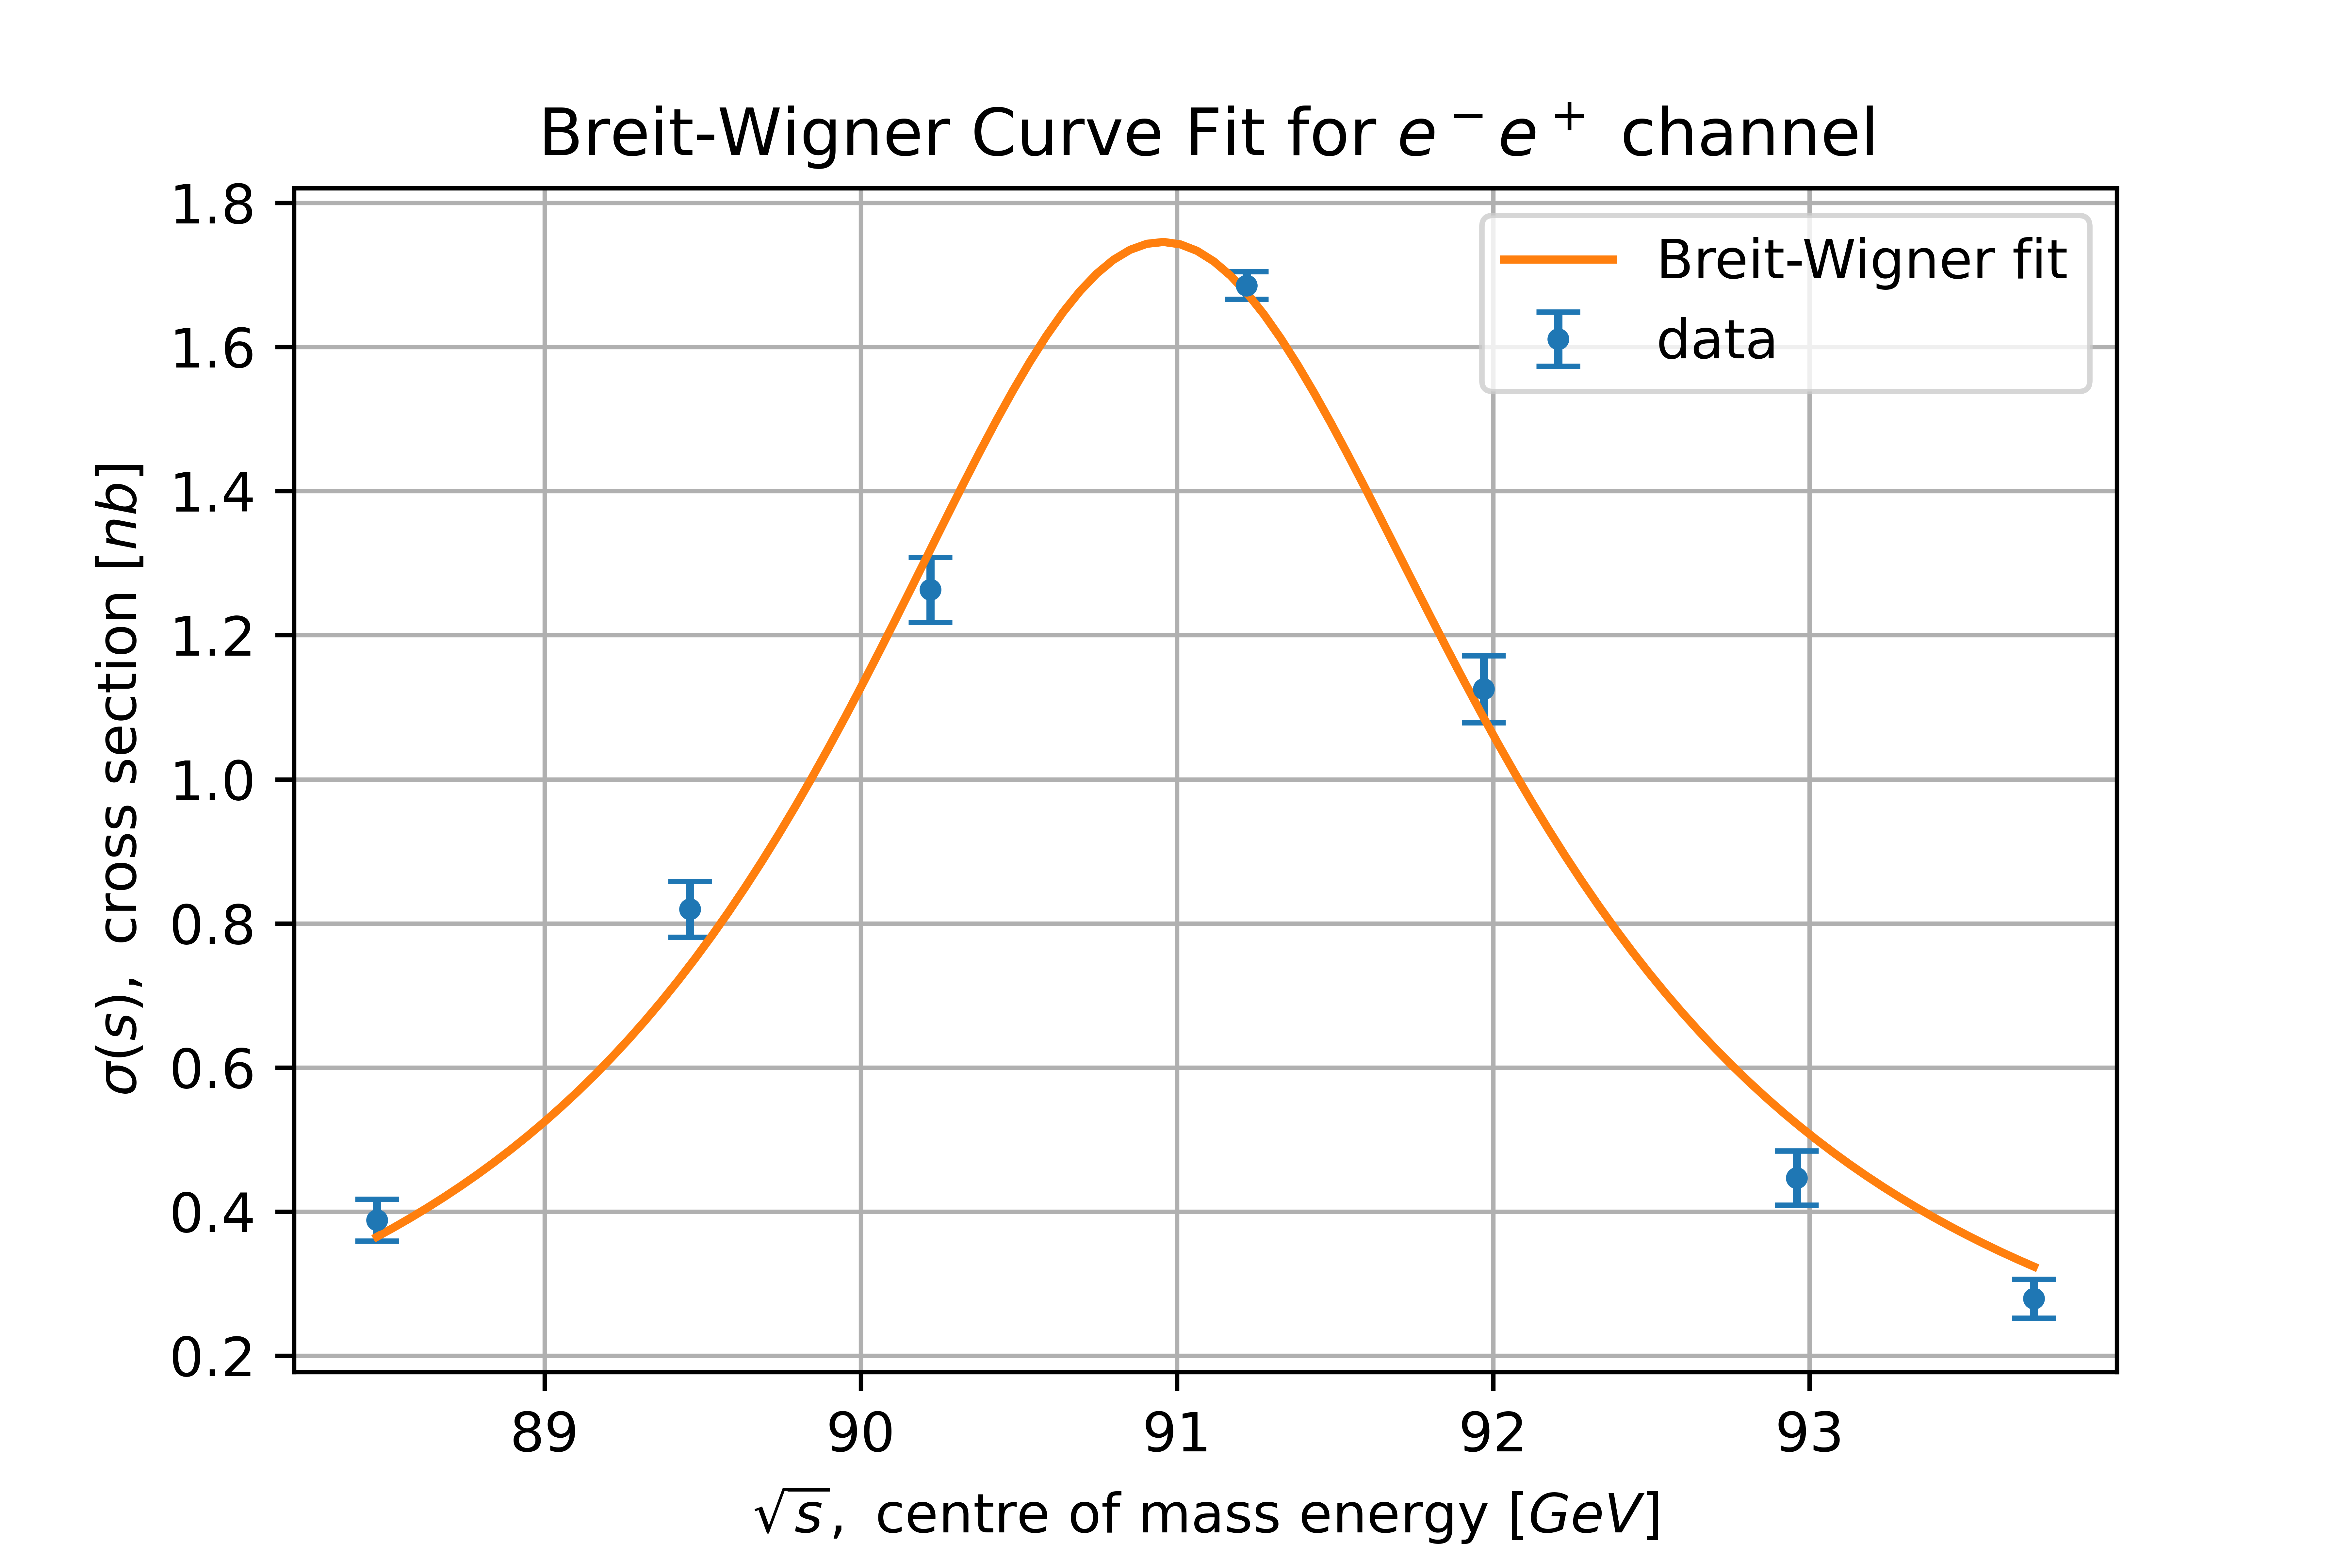
\includegraphics[width = 6 cm]{e213-ee-fit.png}
    
\includegraphics[width = 6 cm]{e213-mm-fit.png}
    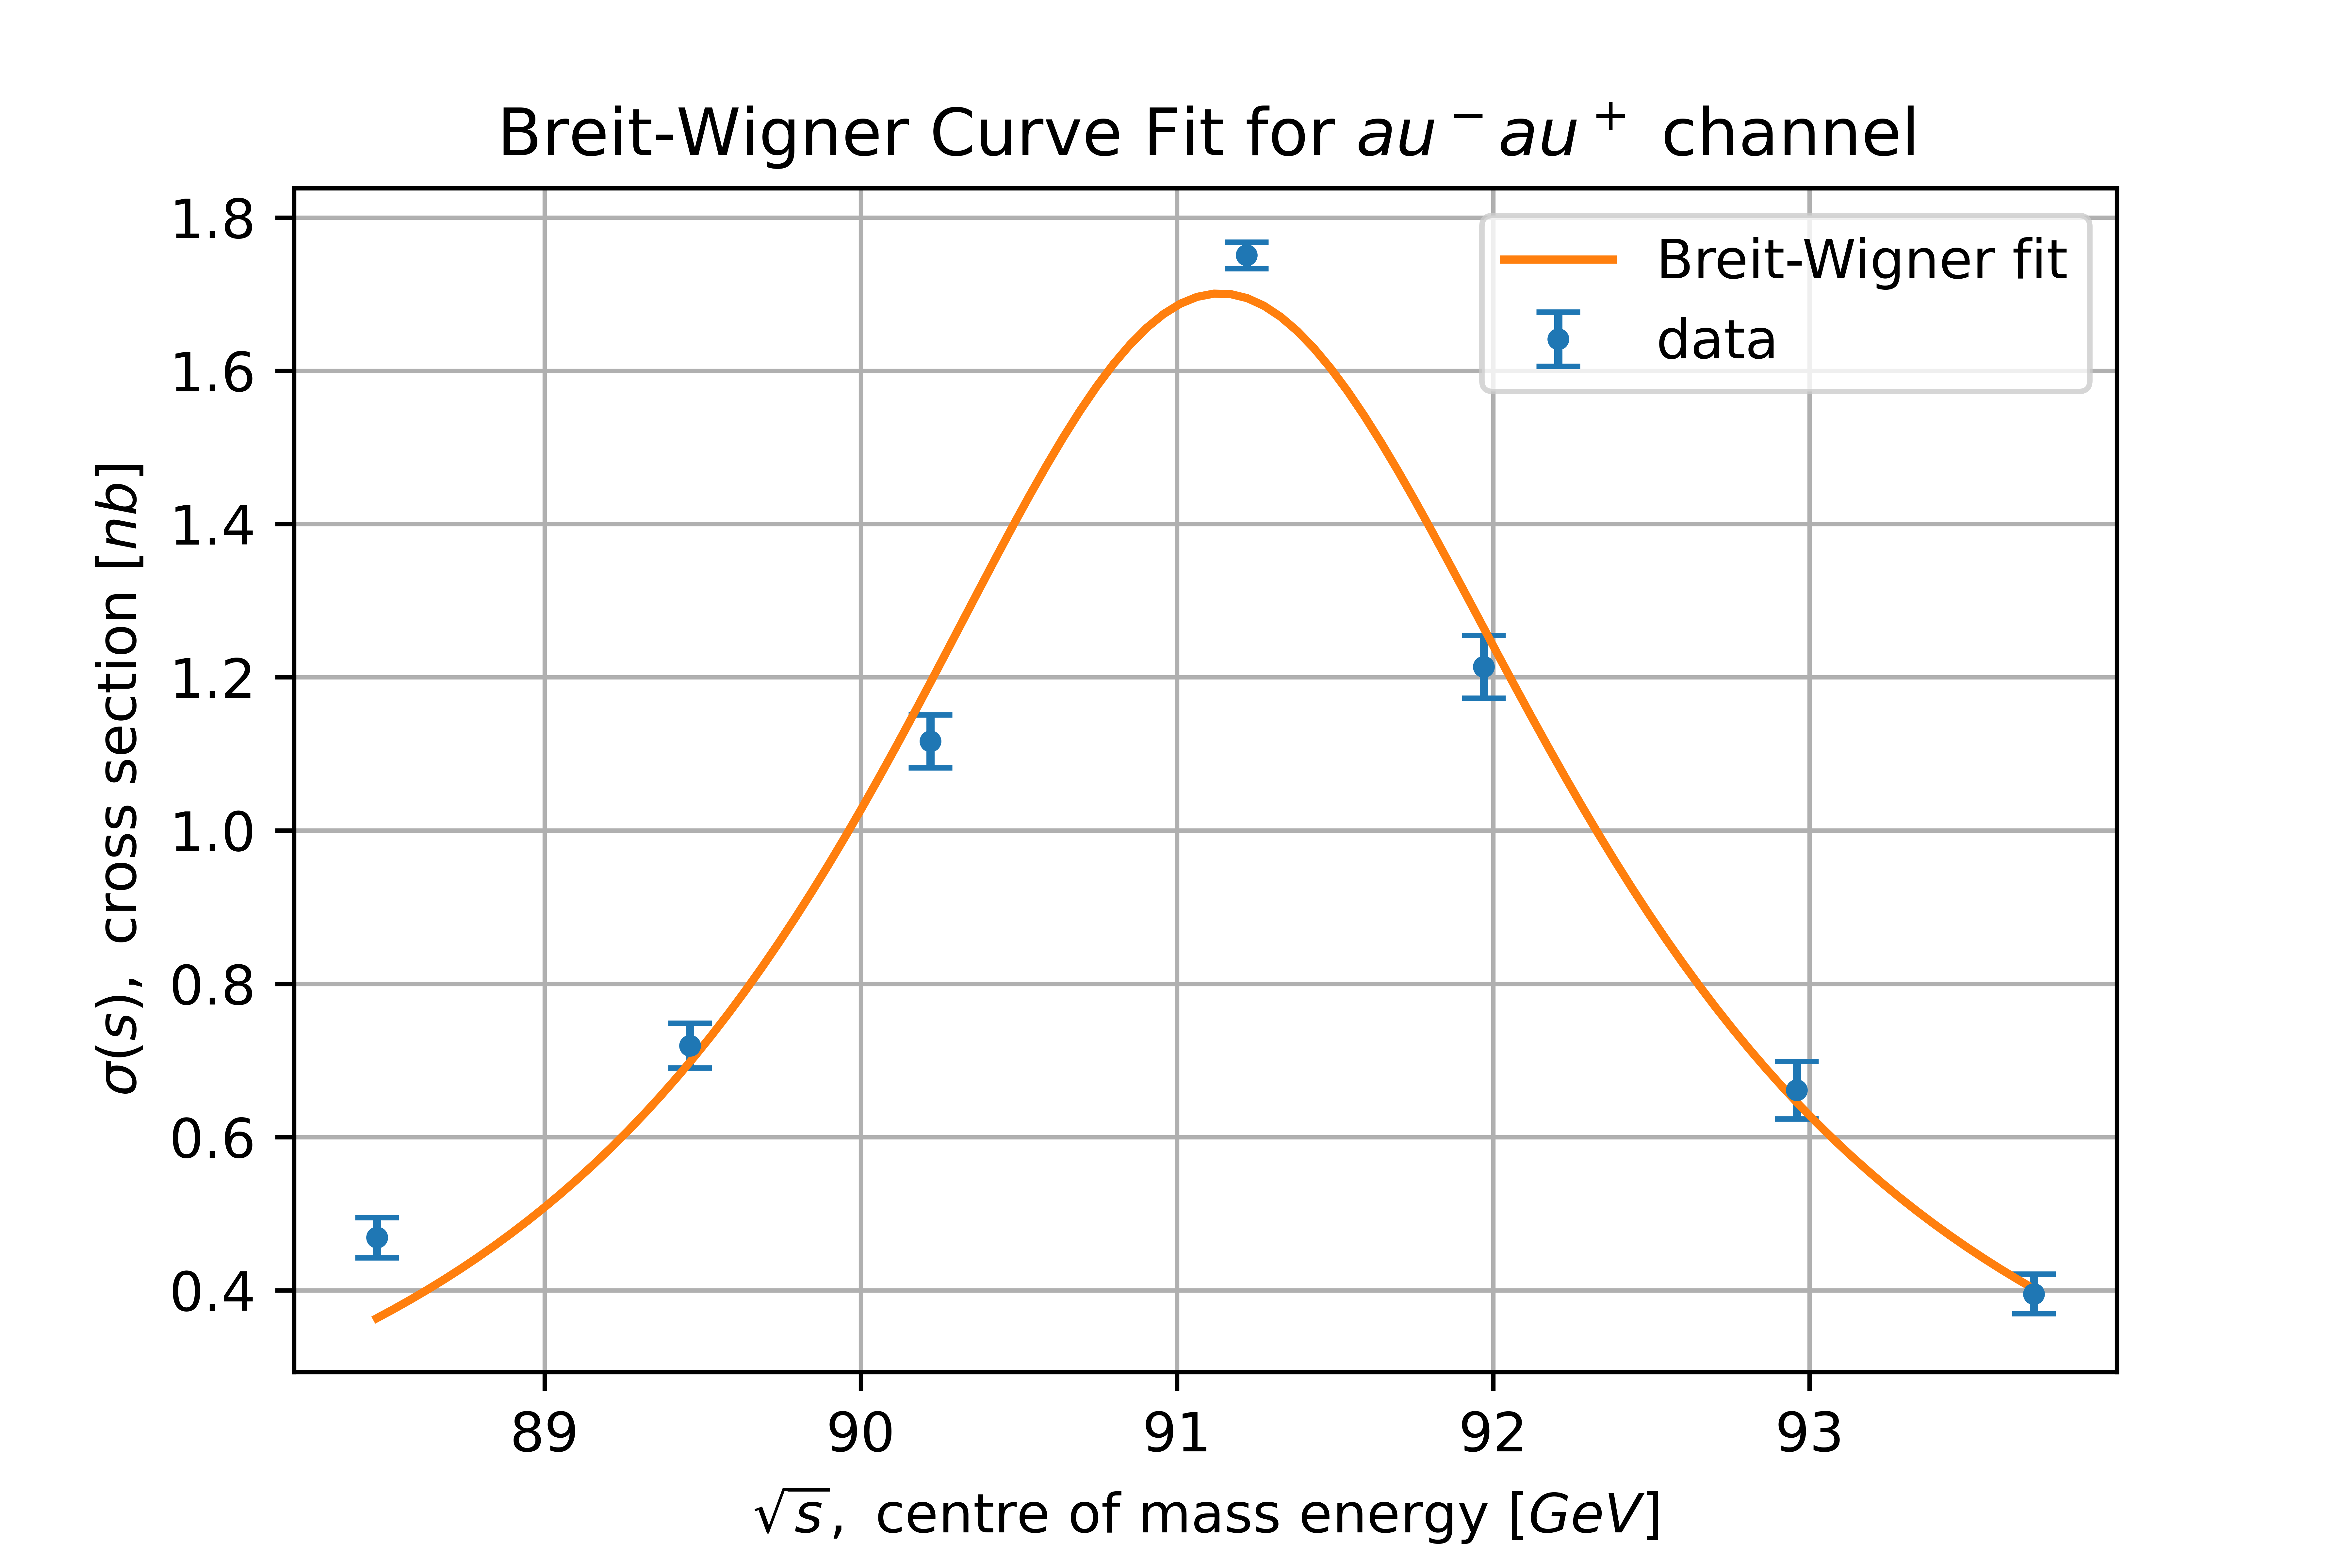
\includegraphics[width = 6 cm]{e213-tt-fit.png}
    
\includegraphics[width = 6 cm]{e213-qq-fit.png}
\end{center}
\caption{Breit-Wigner fit for the four different decay channels}
\label{fig:bwfit}
\end{figure}
\begin{table}[h!]
\centering
\begin{tabular}{c|cccc}
\hline
Channel        & $M_Z$ {[}GeV{]}    & $\Gamma_Z$ {[}GeV{]} & $\Gamma_e\Gamma_f$ {[}GeV$^2${]}                   & $\chi_{red}^2$ \\ \hline
$e^-e^+$       & 90.973 $\pm$ 0.047 & 2.591 $\pm$ 0.158    & 6.615$\times$10$^{-3}$ $\pm$ 6.29$\times$10$^{-4}$ & 3.47           \\
$\mu^-\mu^+$   & 91.117 $\pm$ 0.021 & 2.462 $\pm$ 0.060    & 6.306$\times$10$^{-3}$ $\pm$ 2.46$\times$10$^{-4}$ & 1.10           \\
$\tau^-\tau^+$ & 91.159 $\pm$ 0.058 & 2.825 $\pm$ 0.179    & 7.690$\times$10$^{-3}$ $\pm$ 7.85$\times$10$^{-4}$ & 8.34           \\
$q\bar{q}$     & 91.187 $\pm$ 0.004 & 2.515 $\pm$ 0.010    & 0.1460 $\pm$ 0.0009                                & 0.58          \\ \hline
\end{tabular}
\caption{Fit parameters and reduced $\chi^2$ values for the data}
\label{table:bwfit}
\end{table}
We have three parameters and seven data points. This gives us $4$ degrees of freedom for our fit. The $\mu^-\mu^+$ fit gives the best reduced $\chi^2$ value. The reduced $\chi^2$ value for $q\bar{q}$ is less than 1, which implies that we are over-fitting the data or the error variances are overestimated. The reduced $\chi^2$ value for $e^-e^+$ is greater than 1, which implies that we are under-fitting the data or the error variances are underestimated. Whereas, the reduced $\chi^2$ value for $\tau^-\tau^+$ is much greater than 1, which implies that we don't have a good fit\cite{bevington}. But, none of the fits have a corresponding $p-valule$ less than $0.05$, which means they're not significant enough to be considered seriously different from previous literature results\cite{pvalue}. One major issue with using reduced $\chi^2$ statistic test here is that we have only a limited number of points. Therefore, we don't have a lot of freedom to fit the data with. This ultimately results in a bad value, even though the fit is seemingly nice giving decent values for the parameters. If we had such a good data with more data points, we should obtain a better reduced $\chi^2$ value. Our opinion is that the residuals give a better picture on whether we have a good fit, in our case. And all the residuals here are very small compared to the absolute values that we fit, which means that we have a decent fit for our data. For a better quantitative analysis of goodness of fit, we suggest methods like \textit{bootstrapping}. Reduced $\chi^2$ statistic test is not considered meaningful for limited number of points by some sources\cite{andrae}.\\
The fit parameters directly give us the values of mass of the $Z^0$ boson, $M_Z$ and the decay width of the $Z^0$ boson, $\Gamma_Z$. The mean value of the quantities are,
\begin{equation}
\begin{split}
    M_Z = 91.123 \pm 0.020 \\
    \Gamma_Z = 2.598 \pm 0.062.
\end{split}
\end{equation}
The literature values are $M_Z = 91.1876 \pm 0.0021$ and $\Gamma_Z = 2.4952 \pm 0.0023$ \cite{pdg2}. The literature value for $M_Z$ lies within $4\sigma$ of our calculated value, whereas the literature value for $\Gamma_Z$ lies within $2\sigma$ of our calculated value. We also note that the literature value for $M_Z$ lies within one standard deviation of the value obtained from the $q\bar{q}$ fit, which had the most counts. This hints us that we could improve our accuracy of the results by significantly increasing the number of events analysed.

\subsection{Partial Width of Different Channels and Number of Light Neutrino Generations}
The third fit parameter doesn't directly give us the partial decay width of different channels. It gives the product of the partial decay width of $e^-$ mode and the partial decay width of $f$ mode, the final state fermion in consideration. In the case of $e^-e^+$ channel, this reduces to $\Gamma_e^2$, which lets us calculate the partial decay width of the $e^-$ mode. This can then be used to calculate the partial width of other channels. This is given in the table \ref{table:decaywidth}.\\
\begin{table}[h!]
\centering
\begin{tabular}{c|cc}
\hline
Channel        & $\Gamma_f$ {[}MeV{]} & $\Gamma_f$ (lit.) {[}MeV{]} \\ \hline
$e^-e^+$       & 81.33 $\pm$ 5.47     & 83.91 $\pm$ 0.12              \\
$\mu^-\mu^+$   & 77.53 $\pm$ 6.03     & 83.99 $\pm$ 0.18              \\
$\tau^-\tau^+$ & 94.56 $\pm$ 11.55    & 84.08 $\pm$ 0.22              \\
$q\bar{q}$     & 1795.52 $\pm$ 121.31 & 1744.4 $\pm$ 2.0              \\ \hline
\end{tabular}
\caption{Partial decay width of different channels and literature values}
\label{table:decaywidth}
\end{table}
The literature values for $\Gamma_f$ are taken from \cite{pdg2}. The literature values lie within one standard deviation of the calculated partial width, which is impressive. But we also note that the precision of our results is not as good as the literature value precision. How precise the value of $\Gamma_f$ is, ultimately depends on the precision of the cross section values, which can be improved only by observing more events.\\
With all the decay widths in hand, we can now determine the number of generations of light neutrinos. We use the value for $\Gamma_{\nu}$ from \cite{UB}, which is $\Gamma_{\nu} = 167.6 MeV$. With this, we can calculate the number of neutrino generations using,
\begin{equation}
    n_{\nu} = \frac{\Gamma_Z - \Gamma_e - \Gamma_{\mu} - \Gamma_{\tau} - \Gamma_q}{\Gamma_{\nu}}.
\end{equation}
This gives the number of neutrino generations as,
\begin{equation}
    n_{\nu} = 3.28 \pm 0.45.
\end{equation}
This tells us that number of neutrino generations are $3$. And within one standard deviation, our result absolutely excludes the possibility of fourth neutrino generation.

\subsection{Discussion}

\end{onehalfspace}
\printbibliography

\begin{appendices}
\addtocontents{toc}{\protect\setcounter{tocdepth}{5}}
  \begin{table}[h!]
\centering
\caption{Observed event numbers and actual events numbers for different $\sqrt{s}$ values.}
\begin{tabular}{c|cccc}
\hline
$\sqrt{s}$ {[}GeV{]} & $e^-e^+$      & $\mu^-\mu^+$   & $\tau^-\tau^+$ & $q\bar{q}$       \\ \hline
                     & \multicolumn{4}{c}{$N_{obs}$}                                      \\ \hline
88.47                & 106           & 120            & 251            & 3281             \\
89.46                & 261           & 304            & 425            & 7413             \\
90.22                & 415           & 591            & 693            & 14709            \\
91.22                & 4839          & 8581           & 10178          & 221068           \\
91.97                & 393           & 767            & 863            & 18728            \\
92.96                & 150           & 296            & 427            & 8100             \\
93.71                & 178           & 339            & 459            & 8635             \\ \hline
                     & \multicolumn{4}{c}{$N_{actual}$}                                   \\ \hline
88.47                & 202 $\pm$ 20  & 141 $\pm$ 13   & 256 $\pm$ 18   & 3508 $\pm$ 61    \\
89.46                & 496 $\pm$ 31  & 358 $\pm$ 21   & 416 $\pm$ 23   & 7927 $\pm$ 92    \\
90.22                & 789 $\pm$ 39  & 697 $\pm$ 29   & 661 $\pm$ 30   & 15729 $\pm$ 130  \\
91.22                & 920 $\pm$ 137 & 1023 $\pm$ 111 & 971 $\pm$ 120  & 236399 $\pm$ 541 \\
91.97                & 747 $\pm$ 38  & 904 $\pm$ 33   & 820 $\pm$ 33   & 20026 $\pm$ 147  \\
92.96                & 285 $\pm$ 23  & 349 $\pm$ 20   & 419 $\pm$ 23   & 8662 $\pm$ 96    \\
93.71                & 338 $\pm$ 25  & 400 $\pm$ 22   & 448 $\pm$ 24   & 9234 $\pm$ 100  \\ \hline
\end{tabular}
\label{table:actualnumbers}
\end{table}

\begin{table}[h!]
\centering
\caption{Integrated luminosity values for \textit{data6.root} and radiative and $\text{A}_{\text{FB}}$ corrections for different $\sqrt{s}$ values.}
\begin{tabular}{c|cccc}
\hline
$\sqrt{s}$ {[}GeV{]} & $\int \mathcal{L} dt \text{[nb]}^{-1}$ & \multicolumn{2}{c}{Rad. Correction {[}nb{]}} & $\text{A}_{\text{FB}}$ Correction \\ \hline
                     &                                        & Hadronic              & Leptonic             &                                   \\ \hline
88.47                & 675.9 $\pm$ 5.7                        & +2.0                  & +0.09                & 0.021512                          \\
89.46                & 800.8 $\pm$ 6.6                        & +4.3                  & +0.20                & 0.019262                          \\
90.22                & 873.7 $\pm$ 7.1                        & +7.7                  & +0.36                & 0.016713                          \\
91.22                & 7893.5 $\pm$ 54.3                      & +10.8                 & +0.52                & 0.018293                          \\
91.97                & 825.3 $\pm$ 6.9                        & +4.7                  & +0.22                & 0.030286                          \\
92.96                & 624.6 $\pm$ 5.5                        & -0.2                  & -0.01                & 0.062196                          \\
93.71                & 942.2 $\pm$ 7.7                        & -1.6                  & -0.08                & 0.093850                         \\ \hline
\end{tabular}
\label{table:intlum}
\end{table}
\end{appendices}

\end{document}

